
%!TEX encoding = UTF-8 Unicode
%!TEX root = thesis.tex

 \newif\ifaccess  % test accessibility
 \newif\ifuatwo   % go for UA-2
 \newif\ifoldbib  % use plain old bibliography
 \newif\iftikz
 
 \accesstrue
 \uatwofalse
 \oldbibfalse
 \tikztrue

\ifaccess
    \ifuatwo
        \typeout{USING PDF 2.0/ua-2}
        \DocumentMetadata{
            %check-tagging-status,
            uncompress,
            lang=en-US,
            pdfversion=2.0,
            pdfstandard=a-4f,
            pdfstandard=ua-2,
            tagging=on,
            tagging-setup={math/setup={mathml-SE,mathml-AF}}
            }
          \else
          \typeout{USING PDF 1.7}
          \DocumentMetadata{
            %check-tagging-status,
            uncompress,
            lang=en-US,
            pdfversion=1.7,
            %pdfstandard=a-4f,
            pdfstandard=ua-1,
            tagging=on,
            }
          \fi
    \else
    \typeout{NOT USING TAGPDF}
\fi

\listfiles

\documentclass[onehalf,11pt]{beavtex}
%\documentclass[onehalf,11pt]{book}

\usepackage{fontspec}
\setmainfont{Libertinus Serif}
\setmonofont{Source Code Pro}[Scale=MatchLowercase] 

\usepackage{graphicx}
\usepackage{unicode-math}
\setmathfont[Scale=MatchUppercase]{libertinusmath-regular.otf}

\usepackage[final,babel]{microtype}

% % Figures
% %\usepackage{subfig}
% \usepackage{placeins}

% Tables
% \usepackage{longtable}
\usepackage{booktabs}
% \usepackage{multirow}

% % Math stuff and units
% \usepackage{textcomp,marvosym}
\usepackage{latexsym, amsfonts}  %HMS reenable

%\usepackage{fixmath, upgreek} %provide ISO 80000 conforming greek letters
\usepackage{fixmath} %upgreek is only listed as partially compatible

\usepackage{algorithm}
\usepackage{algpseudocode}

%\usepackage[all,warning]{onlyamsmath} %warns if non-amsmath-environments are used, like $$ ... $$ or eqnarray ... acro.sty must be loaded before this package, otherwise strange error happens!

% \usepackage{framed}
% \usepackage[amsmath,thmmarks,framed]{ntheorem}

% % Acronyms
% %\usepackage{acro}
% %\usepackage[printonlyused]{acronym}

\usepackage{pdflscape}

% \usepackage{adjustbox} % not compatible yet
% \usepackage{afterpage} % not compatible yet
%!TEX encoding = UTF-8 Unicode
%!TEX root = thesis.tex

\definelisting{toc}{TABLE OF CONTENTS}{}{tableofcontents}
\definelisting{lof}{LIST OF FIGURES}{Figure}{listoffigures}
\definelisting{lot}{LIST OF TABLES}{Table}{listoftables}
\definelisting{loa}{LIST OF ALGORITHMS}{Algorithm}{listofalgorithmes}
\definelisting{lol}{LIST OF CODE LISTINGS}{Code}{lstlistoflistings}
\definelisting{loap}{LIST OF APPENDICES}{}{listofappendices}
\definelisting{loaf}{LIST OF APPENDIX FIGURES}{Figure}{listofappendixfigures}
\definelisting{loat}{LIST OF APPENDIX TABLES}{Table}{listofappendixtables}

\usepackage[svgnames]{xcolor}
\definecolor{oregonstateorange}{RGB}{215,63,9}
\definecolor{thedarkblue}{rgb}{0.0,0.0,0.3} 
\definecolor{theblue} {rgb}{0.02,0.04,0.48}
\definecolor{thered}  {rgb}{0.65,0.04,0.07}
\definecolor{thegreen}{rgb}{0.06,0.44,0.08}
\definecolor{thelightgreen}{rgb}{0.06,0.44,0.06}
\definecolor{thegrey} {gray}{0.5}
\definecolor{thegray} {gray}{0.5}
\definecolor{thedarkgray} {gray}{0.95}
\definecolor{theshade}{gray}{0.94}
\definecolor{theframe}{gray}{0.75}
\definecolor{thecream}{rgb}{1,0.95,0.4}
\definecolor{spot}{rgb}{0,0.2,0.6}
\definecolor{boxframe}{gray}{0.8}
\definecolor{boxfill}{rgb}{0.95,0.95,0.99}
\definecolor{theoption}{rgb}{0.118,0.546,0.222}
\definecolor{themacro}{rgb}{0.784,0.06,0.176}
\definecolor{ExampleFrame}{rgb}{0.628,0.705,0.942}
\definecolor{ExampleBack}{rgb}{0.963,0.971,0.994}
\definecolor{Hyperlink}{rgb}{0.281,0.275,0.485}


\usepackage{tikz}
\usetikzlibrary{matrix, positioning}
\usetikzlibrary{calc}

\typeout{ACCESS: USING MYBEAVTEX}
% HMS 2025-10-17 remove biblatex?
\ifoldbib
    %\usepackage[nottoc,numbib]{tocbibind} beavtex did not use this
    \typeout{ACCESS: USING OLD BIB STYLE}
\else
    \typeout{ACCESS: USING NEW BIB STYLE}
    \usepackage[maxbibnames=99, sorting=none, backend=biber, style=numeric]{biblatex} % load the package
    % HMS change to sorting=none
    %\ExecuteBibliographyOptions{doi=false, eprint=false} % only works with numeric style
    \ExecuteBibliographyOptions{doi=true, eprint=true} % HMS turn these on
    % have biblatex showing [?] instead of the stupid bibtex key
    \makeatletter
    \def\blx@citeadd#1{%
    	\ifcsdef{blx@keyalias@\the\c@refsection @#1}
    	{\edef\blx@realkey{\csuse{blx@keyalias@\the\c@refsection @#1}}}
    	{\def\blx@realkey{#1}}%
    	\expandafter\blx@getrefcontext\expandafter{\blx@realkey}% needed for \ifdata
    	\expandafter\blx@citation\expandafter{\blx@realkey}\blx@msg@cundefon
    	\expandafter\blx@ifdata\expandafter{\blx@realkey}
    	{\advance\blx@tempcnta\@ne
    		\listeadd\blx@tempa{\blx@realkey}}
    	{\ifnum\blx@tempcntb>\z@\multicitedelim\fi
    		\expandafter\abx@missing\expandafter{?}%<- the change is here
    		\advance\blx@tempcntb\@ne}}
    \makeatother
\fi

%\pdfinterwordspaceon

\title{A Very Long Example Title: For the Purpose of Demonstrating that Underlining Works Despite an Excessively Long Title}

\author{Benny Beaver}
\degree{Master of Science}
\doctype{Thesis}
\department{Electrical Engineering and Computer Science}
\depttype{School}
\depthead{Director}
\major{Electrical and Computer Engineering}
\advisor{Vincent Immler}
\submitdate{Oct 22, 2025}
\commencementyear{2025}

\abstract{
Here you put the text for your abstract (motivation, problem statement, approach, results, conclusion, impact).
This template \emph{requires} LuaLaTeX 2025-11-01 (or simply TeXLive 2026).
It is designed to pass digital accessibility checks but you will still be required to check the result to confirm.
The base class of this template is `book' which supports hierarchical structures based on: parts, chapters, sections, subsections, subsubsection and paragraph.
You may want to use parts only for a dissertation with additional minitoc \href{https://mediatum.ub.tum.de/doc/1482457/document.pdf}{as demonstrated in my dissertation}.
For references, please use biblatex with biber as backend (not the outdated bibtex).
\textbf{Please also note: this is currently set to use Libertine (Libertinus) font with the intention to use Source Code Pro for verbatim environments (as a quick workaround for the lack of lstlisting).}
\textcolor{oregonstateorange}{Go Beavs!}
}

\acknowledgements{Creating this thesis template has been a collaborative effort by multiple people affiliated with Oregon State University: Heidi Schellmann, David A Craig, Ross Hatton, and Vincent Immler.}

\ifoldbib
   % VI: I do not recommend using bibtex anymore; only biblatex with biber; consider this a legacy option
\else
    \addbibresource{thesisbib.bib}
    % adding multiple .bib files is possible
    %\addbibresource{youradvisorsfavorite.bib}
    %\addbibresource{yourfriendsfavorite.bib}
\fi

\makeatletter
\AtBeginDocument{
	\hypersetup{
		pdftitle = {\@title},
		pdfauthor = {\@author},
		pdfsubject={\@title},
		pdfkeywords={Oregon State University}
	}
}
\makeatother

\usepackage{hyperref}

\hypersetup{
pdflang={en-US},
pdfdisplaydoctitle=true,
	unicode=true,
	colorlinks=true,
	linkcolor=thedarkblue,
	citecolor=thegreen,
	filecolor=black,
	urlcolor=thedarkblue,
	%	backref=section,
	%bookmarksopen=true,
	%bookmarksopenlevel=3,
	%bookmarksdepth=subsection,
	hypertexnames=false,
	linktocpage=true,
	plainpages=false,
	breaklinks
}

\ifpdf
	\hypersetup{linktocpage=false} % false=links are section names, true=links are page numbers
\else
	\hypersetup{linktocpage=true} % false=links are section names, true=links are page numbers
	\usepackage[hyphenbreaks]{breakurl}
\fi

% used for acro package
%\usepackage[macros=true, xspace=true]{acro}
%%!TEX encoding = UTF-8 Unicode
%!TEX root = thesis.tex

% \DeclareAcronym{sca}{short = SCA ,long  = Side Channel Analysis,tag = abbrev}
% \DeclareAcronym{XOR} {short = $\oplus$,long = Binary XOR-Operation,tag = symbols}

% \DeclareAcronym{AWG} {short = AWG,long = Arbitrary Waveform Generator,tag = abbrev}
% \DeclareAcronym{OPAMP} {short = OPAMP,long = Operational Amplifier,tag = abbrev}
% \DeclareAcronym{PDN} {short = PDN,long = Power Delivery Network,tag = abbrev}
% \DeclareAcronym{DUT} {short = DUT,long = Device Under Test,tag = abbrev}


%\usepackage{subcaption}
%\captionsetup{compatibility=false}

\usepackage{fancyvrb}
\usepackage{tcolorbox}

%!TEX encoding = UTF-8 Unicode
%!TEX root = thesis.tex

% for annotations
\newcommand*\numcircledtikz[1]{\tikz[baseline=(char.base)]{
		\node[shape=circle,draw,inner sep=1.2pt] (char) {#1};}} 

% properly scaled \texttt command
\let\oldtexttt\texttt% Store \texttt
\renewcommand{\texttt}[1]{{\small \ttfamily #1}}


\DefineVerbatimEnvironment{coding}{Verbatim}{numbers=left,fontsize=\small}


% verbatim environment with SourceCodePro
\makeatletter 
%  \def\verbatim@font{\fontfamily{SourceSansPro-TOsF}\footnotesize% select the font 
\def\verbatim@font{\fontfamily{SourceCodePro-TOsF}\footnotesize% select the font 
\let\do\do@noligs 
\verbatim@nolig@list} 
\makeatother

% for commands, filenames, etc. within text
\DefineVerbatimEnvironment{VerbOutPlainSource}{Verbatim}{fontfamily=SourceCodePro-TOsF,fontsize=\small}
\def\code#1{{\fontfamily{SourceCodePro-TOsF}\selectfont\small #1}}
%!TEX encoding = UTF-8 Unicode
%!TEX root = thesis.tex

% \DeclarePairedDelimiter\ceil{\lceil}{\rceil}
% \DeclarePairedDelimiter\floor{\lfloor}{\rfloor}

% \DeclareMathOperator{\Throughput}{\mathrm{Throughput}}
% \DeclareMathOperator{\StoredData}{\mathrm{Stored\, Data}}
% \DeclareMathOperator{\var}{\mathrm{var}}
% \DeclareMathOperator{\cov}{\mathrm{cov}}

\newcommand{\dH}{\ensuremath{\mathrm{d}_{\mathrm{H}}\xspace}}
%\newcommand{\dA}{\ensuremath{\mathrm{d}_{\mathrm{A}}\xspace}}
\newcommand{\dE}{\ensuremath{\mathrm{d}_{\mathrm{E}}\xspace}}
\newcommand{\dHB}{\ensuremath{\mathrm{d}_{\mathrm{H}|2}\xspace}}
\newcommand{\dHS}{\ensuremath{\mathrm{d}_{\mathrm{H}|S}\xspace}}
\newcommand{\dLee}{\ensuremath{\mathrm{d}_{\mathrm{Lee}}\xspace}}
\newcommand{\dLev}{\ensuremath{\mathrm{d}_{\mathrm{Lev}}\xspace}}
\newcommand{\dMan}{\ensuremath{\mathrm{d}_{\mathrm{Man}}\xspace}}

\newcommand{\hdA}{\ensuremath{\prescript{\mathrm{A}}{}{W}}}
\newcommand{\hdQ}{\ensuremath{\prescript{\mathrm{Q}}{}{W}}}
\newcommand{\hdE}{\ensuremath{\prescript{\mathrm{ECC}}{}{W}}}

\newcommand{\hdAw}{\ensuremath{\prescript{\mathrm{A}}{}{w}}}
\newcommand{\hdQw}{\ensuremath{\prescript{\mathrm{Q}}{}{w}}}
\newcommand{\hdEw}{\ensuremath{\prescript{\mathrm{ECC}}{}{w}}}
		
%\newcommand{\TSn}{\ensuremath{\mathrm{TS}_{\mathrm{node}}\xspace}}
\newcommand{\TSn}[1][]{\ensuremath{\mathrm{TS}_{\mathrm{node}}^{\mathrm{#1}}\xspace}}
%\newcommand{\TSd}{\ensuremath{\mathrm{TS}_{\mathrm{device}}\xspace}}
\newcommand{\TSd}[1][]{\ensuremath{\mathrm{TS}_{\mathrm{device}}^{\mathrm{#1}}\xspace}}

% \DeclareMathOperator{\bit}{\ensuremath{\xspace\mathrm{bit}}}
% \DeclareMathOperator{\bits}{\ensuremath{\xspace\mathrm{bits}}}
% \DeclareMathOperator{\bps}{\ensuremath{\xspace\mathrm{bits/segment}}}

\newcommand{\MI}[1]{\ensuremath{\mathrm{I}(#1)}\xspace}
\newcommand{\AVG}[1]{\ensuremath{\mathrm{E}(#1)}\xspace}
\newcommand{\IRS}[1]{\ensuremath{\mathrm{IRS}(#1)}\xspace}
\newcommand{\RS}[1]{\ensuremath{\mathrm{RS}(#1)}\xspace}
\newcommand{\BCH}[1]{\ensuremath{\mathrm{BCH}(#1)}\xspace}
\newcommand{\VT}[1]{\ensuremath{\mathrm{VT}(#1)}\xspace}
\newcommand{\LMC}[1]{\ensuremath{\mathrm{LMC}(#1)}\xspace}
\newcommand{\enc}[1]{\ensuremath{\mathrm{enc}(#1)}\xspace}

\newcommand{\txe}[1]{$\mathrm{Tx}_{#1}$}
\newcommand{\rxe}[1]{$\mathrm{Rx}_{#1}$}
\newcommand{\txer}[1]{$\mathrm{Tx}_{#1}\mathrm{R}$}
\newcommand{\rxer}[1]{$\mathrm{Rx}_{#1}\mathrm{R}$}
% \DeclareMathOperator{\ld}{\mathrm{ld}}
% \DeclareMathOperator{\hd}{\mathrm{HD}}

\newcommand{\pn}{{P}_\mathrm{n}}
\newcommand{\ps}{{P}_\mathrm{s}}
\newcommand{\pd}{{P}_\mathrm{d}}
\newcommand{\hpn}{\hat{P}_\mathrm{n}}
\newcommand{\hps}{\hat{P}_\mathrm{s}}
\newcommand{\hpd}{\hat{P}_\mathrm{d}}

\newcommand{\WQ}{W_{\mathrm{Q}}}

\newcommand{\NP}{\textsc{np}}
\newcommand{\T}{\textsc{true}}
\newcommand{\F}{\textsc{false}}


\newcommand{\iid}{i.i.d.\xspace}
\newcommand{\eg}{e.g., }
\newcommand{\ie}{i.e., }
\newcommand{\etal}{et al. }
\newcommand{\etc}{etc.~}
\newcommand{\Sbox}{S-box}
\newcommand{\Fig}{Fig.}

\newcommand{\GF}[1]{\ensuremath{\mathrm{GF}(#1)}\xspace}
%\newcommand{\GF}[1]{\ensuremath{\mathbb{F}_{#1}}\xspace}
\newcommand{\GFQ}{\GF{q}}
\newcommand{\N}{\ensuremath{\mathbb{N}}\xspace}

\newcommand{\QsquaredsubQE}{Q^2_{QE}}

\newcommand{\chisquared}{\chi^2}
\newcommand{\pperp}{p_{T}}
\newcommand{\ppar}{p_{||}}


% make certain tagpdf knows about the table format
\ifaccess
\tagpdfsetup{table/header-rows={1}}
\fi

\begin{document}
\frontmatter
\pagestyle{empty}

%\flyleaf

%!TEX encoding = UTF-8 Unicode
%!TEX root = ../thesis.tex
\typeout{ACCESS - ABSTRACT \thepage}
%\cleardoublepage
%\addcontentsline{toc}{section}{Abstract}
%\addchap*{Abstract}
%\adjustmtc % adjust minitoc

% Motivation
% Problem statement
% Approach
% Results
% Conclusion

\abspage

%\thispagestyle{empty}
%\cleardoublepage
%!TEX encoding = UTF-8 Unicode
%!TEX root = ../thesis.tex
\typeout{ACCESS - COPYRIGHT PAGE \thepage }
%\cleardoublepage
%\addcontentsline{toc}{section}{Imprint}

\begin{singlespacing}
	\thispagestyle{empty}
	\vspace*{10\baselineskip}
	\begin{center}
		\makeatletter
		{\textcopyright} Copyright by \@author\\
		\@submitdate \\
		All Rights Reserved
		\makeatother
	\end{center}
\end{singlespacing}

\newpage

%!TEX encoding = UTF-8 Unicode
%!TEX root = ../thesis.tex
\typeout{ACCESS - TITLE PAGE \thepage}
\begin{titlepage}
	
    \thispagestyle{empty}
	\begin{center}
	\makeatletter
	\setlength{\baselineskip}{14.5pt}
	{\heading \@title} \\
	\emptyline by\\ \emptyline
	\@author\\
	\vfill
	A \MakeUppercase{\@doctype}\\ \emptyline
	submitted to\\ \emptyline
	Oregon State University\\
	\vfill
	in partial fulfillment of\\
	the requirements for the\\
	degree of\\ \emptyline
	\@degree
	\vfill
	Presented \@submitdate\\
	Commencement June \@commencementyear
	\makeatother
\end{center}
\newpage

\end{titlepage}

%!TEX encoding = UTF-8 Unicode
%!TEX root = ../thesis.tex
\typeout{ACCESS - APPROVALPAGE \thepage}
%\cleardoublepage
%\addcontentsline{toc}{section}{Preface}
%\vspace*{1mm}

%\thispagestyle{empty}
%\newlength\longest
%\null\vfill

  \thispagestyle{empty}
\begin{singlespacing}
	\begin{flushleft}
		\makeatletter
		\noindent
		\ulinewithbreaks{\@degree} \MakeLowercase{\@doctype} of \ulinewithbreaks{\@author} 
		presented on \uline{\@submitdate}. \\
		\vspace{3em}
		APPROVED:\\
		\vspace{3em}
		\hrulefill \\
		% Major Professor (Co- if there is a coadvisor}
	\if\@coadvisor *
	\else Co-\fi Major Professor, representing \@major \\
	\vspace{3em}
	% Second major professor if exists
	\if\@coadvisor *
	\else\hrulefill \\  Co-Major Professor, representing \@twomajor \\
	\vspace{3em}
	\fi
	\hrulefill \\ 
	% major department head
	\@depthead\ of the \@depttype\ of \@department \\
	\vspace{3em}
	\if\@twodepartment * 
	\else
	% Here is the second Department
	\hrulefill \\ 
	\@twodepthead\ of the \@twodepttype\ of \@twodepartment \\
	\vspace{3em}
	\fi
	\hrulefill \\
	Dean of Graduate Education \\
	\vfill
	I understand that my \MakeLowercase{\@doctype} will become part of the
	permanent collection of Oregon State University libraries. My signature
	below authorizes release of my \MakeLowercase{\@doctype} to any reader
	upon request.
	\vspace{3em} \\
	\hrulefill \\
	\makebox[\textwidth]{\hfill \@author, Author \hfill}
	\makeatother
\end{flushleft}
\end{singlespacing}
\newpage
  %HMS replace uline with underline - problem for long titles. 
%!TEX encoding = UTF-8 Unicode
%!TEX root = ../thesis.tex
\typeout{ACCESS - ACKNOWLEGEMENTS \thepage}
%\cleardoublepage
%\addcontentsline{toc}{section}{Acknowledgements}
%\addchap*{Acknowledgements}
%\adjustmtc % adjust minitoc

\ackpage 

%\cleardoublepage



%\addtocontents{toc}{\protect\markboth{\contheading}{\contheading}}
%\microtypesetup{protrusion=false}
%\addcontentsline{toc}{chapter}{Table of Contents} % currently messes up minitoc
%\renewcommand{\contentsname}{\hspace*{\fill}\bfseries\Large Contents\hspace*{\fill}} % center "Contents"
%\addcontentsline{toc}{section}{Table of Contents} % bookmark does not work properly, page number is correct though
%https://tex.stackexchange.com/questions/363998/remove-or-change-the-zero-before-table-of-contents
\typeout{ACCESS - TABLE OF CONTENTS \thepage}
\tableofcontents
%\microtypesetup{protrusion=true}

%% generate list of figures
\newpage
%\addcontentsline{toc}{chapter}{List of Figures}
\typeout{ACCESS - LIST OF FIGURES \thepage}
\listoffigures
\newpage

%% generate list of tables
\newpage
%\addcontentsline{toc}{chapter}{List of Tables}
\typeout{ACCESS - LIST OF TABLES \thepage}
\listoftables

% %% generate list of algorithms
 %\newpage
%\addcontentsline{toc}{chapter}{List of Algorithms}
%\listofalgorithms
% \listofalgorithmes % for algo2e: not a typo, algo2e option redefines \listofalgorithms into \listofalgorithmes
%\clearpage

% %% generate list of code listings
% \newpage
% \lstlistoflistings
% \clearpage

\typeout{ACCESS - BEFORE MAIN MATTER}
\mainmatter
\part{Thesis} %comment this HC or MS thesis; suggest to keep for PhD

%!TEX encoding = UTF-8 Unicode
%!TEX root = ../thesis.tex

\typeout{ACCESS - INTRODUCTION \thepage}
\chapter{Introduction}\label{ch:introduction}

Motivation and problem statement (if longer: make it separate sections)

\section{Related Work}\label{sec:related_work}

\section{Contribution}\label{sec:contribution}

\section{Outline}\label{sec:outline}


%!TEX encoding = UTF-8 Unicode
%!TEX root = ../thesis.tex

\typeout{ACCESS - BACKGROUND}
\chapter{Background}\label{ch:background}

\typeout{ACCESS - NEW SECTION 1}
\section{Notes on Accessibility}

\section{Basic Mathematical Expressions}\label{sec:intro_math}

%If $x$ is real, then $x^{2} \geq 0$.

A matrix equation.
\[
\begin{pmatrix}0&1\\1&0\end{pmatrix}
\begin{pmatrix}a&b\\c&d\end{pmatrix}
=
\begin{pmatrix}c&d\\a&b\end{pmatrix}
\]

%!TEX encoding = UTF-8 Unicode
%!TEX root = ../thesis.tex

\chapter{Implementation of xxx}


\section{Concept for xxx}\label{sec:concept-wave}


\section{Actual Implementation}\label{sec:actual-implementation}


%!TEX encoding = UTF-8 Unicode
%!TEX root = ../thesis.tex

\typeout{ACCESS - MEASUREMENT SETUP \thepage}
\chapter{Measurement Setup}\label{chap:measure}

Just putting some stuff here \dots

\begin{figure}[htbp]
\centering
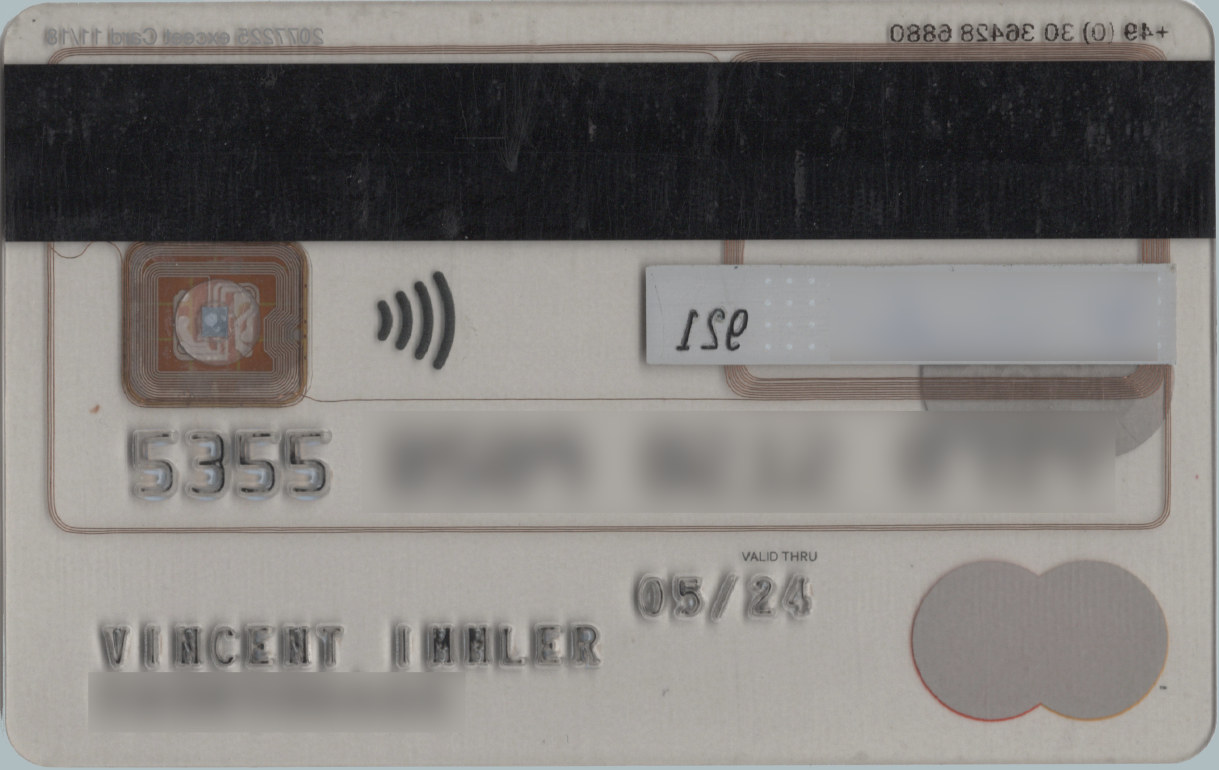
\includegraphics[height=4cm,alt={Credit card.}]{figures_internal/credit_card_alternative_crop_scaled}
\caption{Example figure with alt text for accessibility.}
\label{fig:creditcard}
\end{figure}
%!TEX encoding = UTF-8 Unicode
%!TEX root = ../thesis.tex

\chapter{Practical Results}\label{chap:results}

\section{Results 1}\label{sec:results1}

\section{Results 2}\label{sec:results2}



%!TEX encoding = UTF-8 Unicode
%!TEX root = ../thesis.tex

\chapter{Conclusion}

\section{Summary}

\section{Future Work}


\part{Accessibility Tests} % remove this part and subsequent tests for use
%!TEX encoding = UTF-8 Unicode
%!TEX root = ../thesis.tex

\typeout{ACCESS - CHECKLIST}
\chapter{Requirements}\label{ch:requirements}

Here are things we need to include in our test suite to emulate a real thesis

\section{For all Theses}\label{sec:rec_all_theses}
\begin{enumerate}%[label={$\square$}]   % this gives untagged figure in Canvas so revert
\item test figure captions and references to figures as in Figure \ref{fig:creditcard}. The test is in Chapter \ref{ch:background}.
\item test complete mathematical formulas, see Chapter \ref{ch:testmath}
\item test putting tables in both the main body and appendices as shown in Chapter \ref{ch:testtable} and Appendix \ref{ch:testappendixtable}.
\item test cross chapter referencing.
\end{enumerate}

\begin{enumerate}
\item One
\item Two
\item Three
\end{enumerate}

\begin{itemize}
\item item
\item item
\item item
\end{itemize}

\section{Testing Software}\label{sec:req_testing}

\begin{enumerate}
    \item Canvas
    \item Adobe Acrobat Professional -- accessibility checker and preflight
    \item veraPDF tests for conformity to ISO Standard 32005
\end{enumerate}
%!TEX encoding = UTF-8 Unicode
%!TEX root = ../thesis.tex
\typeout{ACCESS - TEST LISTING \thepage}

\chapter{Test Code Listings} \label{chap:codelistings}

\section{Example: Verbatim Listing} \label{sec:verbatimlistings}

For now, the \LaTeX\/ package \texttt{listing} is not compatible with tagging which is why we will use the plain verbatim environment.
The first code snippet is just using a plain verbatim environment:

\begin{verbatim}
#include <stdio.h>

int main() {
    printf("Hello, World!\n");
    return 0;
}
\end{verbatim}

The second code snippet is using a custom verbatim environment with the Adobe Source Code Pro font and line numbers:

\begin{coding}
#include <stdio.h>

int main() {
    printf("Hello, World!\n");
    return 0;
}
\end{coding}



\section{Example: Verbatim combined with tcolorbox Listing} \label{sec:tcolorboxlistings}

Additionally requires the package \texttt{tcolorbox}.

\begin{tcolorbox}[colback=gray!25, boxsep=0pt, arc=0pt, boxrule=0pt]
\begin{coding}
#include <stdio.h>

int main() {
    printf("Hello, World!\n");
    return 0;
}
\end{coding}
\end{tcolorbox}

\section{Example: Code Listing with Listings}

(underlying package not compatible yet)

% \begin{lstlisting}[language=C, caption={Firmware for instruction skipping.}, label=lst:stmdut]
%     uint32_t glitched = 0x01u;
%     sigTermInit();
%     sigEnabOne();

%     while (glitched) //THIS INSTRUCTION CAN BE GLITCHED
%     {
%     ;
%     }
%     // Increment instruction skip counter
%     glitched++;
%     glitched++;
%     asm("NOP");
%     asm("NOP");
%     asm("NOP");
%     asm("NOP");
%     asm("NOP");
%     asm("NOP");

%     while (glitched)
%     {
%         if (glitched == 0x01u) {
%             sigTermOne();
%             sigEnabTwo();
%         } else if (glitched == 0x02u) {
%             sigTermOne();
%             sigTermTwo();
%         } else if (glitched == 0x03u) {
%             sigEnabOne();
%             sigEnabTwo();
%         }
%     }
% \end{lstlisting}
%!TEX encoding = UTF-8 Unicode
%!TEX root = ../thesis.tex

\typeout{ACCESS - TESTMATH \thepage}
\chapter{Gnarly Math}\label{ch:testmath}

\section{Example by Ulrike Fischer}\label{sec:test_math_example}
This example was shown in reference \cite{ctan:tagpdftalk}.
\begin{align}
f(x) &= |{x}| +
\begin{cases}
1 & \text{if $x<0$} \\
0 & \text{if $x=0$} \\
-1 & \text{if $x>0$}
\end{cases}\label{A} \\
%
f(x) &> -1 \quad \text{see \eqref{A}}
\end{align}

\section{Checking Macros}

I type this a lot $\QsquaredsubQE$.

\section{More Math}

\newcommand{\melt}[3]{\ensuremath{\langle {#1} | {#2} | {#3} \rangle}}

The  Hadamard propagator can then be written as 
\begin{equation} \label{eq:vertexexp}
G^\pm_{\mathrm{H}}(\nu_f,\phi_f;\nu_i,\phi_i) =
\sum_{M=0}^{\infty} \sum_{ \substack{\nu_{M-1},\ldots,\nu_1\\ \nu_m\neq \nu_{m+1}}}
A^{\pm}_M(\nu_{M},\nu_{M-1},\ldots,\nu_{1},\nu_{0};\Delta\phi) ,
\end{equation} 
(Same equation using eqnarray and subequations:
\begin{subequations}
\begin{eqnarray}
G^\pm_{\mathrm{H}}(\nu_f,\phi_f;\nu_i,\phi_i) 
% % #1\atop #2
%  & = &
% \sum_{M=0}^{\infty} \sum_{{\nu_{M-1},\ldots,\nu_1}\atop{\nu_m\neq \nu_{m+1}}}
% A^{\pm}_M(\nu_{M},\nu_{M-1},\ldots,\nu_{1},\nu_{0};\Delta\phi)   \\
%  & = &
% % \substack{#1\\ #2} produces larger output that atop
% \sum_{M=0}^{\infty} \sum_{\substack{\nu_{M-1},\ldots,\nu_1\\ \nu_m\neq \nu_{m+1} }}
% A^{\pm}_M(\nu_{M},\nu_{M-1},\ldots,\nu_{1},\nu_{0};\Delta\phi)   \\
 & = &
% \genfrac{}{}{0pt}{}{#1}{#2} produces output simialr to atop
\sum_{M=0}^{\infty} \sum_{\genfrac{}{}{0pt}{}{\nu_{M-1},\ldots,\nu_1}{\nu_m\neq \nu_{m+1} }}
A^{\pm}_M(\nu_{M},\nu_{M-1},\ldots,\nu_{1},\nu_{0};\Delta\phi)   \\
 & = &
\sum_{M=0}^{\infty} \sum_{{\nu_{M-1},\ldots,\nu_1}}
P^{\pm}_M(\nu_{M},\nu_{M-1},\ldots,\nu_{1},\nu_{0};\Delta\phi)
\end{eqnarray}
\end{subequations}
where the ``path amplitude'' $A^{\pm}_M$ associated with the path
$(\nu_{M},\nu_{M-1},\ldots,\nu_{1},\nu_{0})$ is given in terms of the matrix 
elements $\Theta_{\nu\nu'}=\melt{\nu}{\Theta}{\nu}$ by %
% \footnote{There is a similar alternative expansion for $G^\pm_{\mathrm{NW}}$
% in terms of the matrix elements of $H=\sqrt{\Theta}$.
% } %
\begin{multline}
A^{\pm}_M(\nu_{M},\nu_{M-1},\ldots,\nu_{1},\nu_{0};\Delta\phi)  =
\Theta_{\nu_M\nu_{M-1}}\ldots\Theta_{\nu_2\nu_1}\Theta_{\nu_1 \nu_0}  \\
\times\prod_{k=0}^{p-1}\frac{1}{(d_k-1)!} \left(\frac{\partial}{\partial \Theta_{w_k w_k}}\right)^{d_k-1}
\sum_{l=0}^{p-1} \frac{e^{\pm i\sqrt{\Theta_{w_l w_l}}\Delta\phi}}{2\sqrt{\Theta_{w_l w_l}}
%      \prod_{ {j=0}\atop{j\neq l}}^{p-1} (\Theta_{w_l w_l}-\Theta_{w_j w_j})}.
       \prod_{ \substack{j=0\\ j\neq l}}^{p-1} (\Theta_{w_l w_l}-\Theta_{w_j w_j})}.
%      \prod_{ \genfrac{}{}{0pt}{}{j=0}{j\neq l}}^{p-1} (\Theta_{w_l w_l}-\Theta_{w_j w_j})}.
\end{multline}
(I have worse if we need them.)


%!TEX encoding = UTF-8 Unicode
%!TEX root = ../thesis.tex


\typeout{ACCESS - TESTTABLE \thepage}

\chapter{Test of a Table}\label{ch:testtable}


\begin{table}[ht]
    \begin{centering}
    \begin{tabular}{c c l}
    
    %\hline
   
    \bf
    Time&\qquad \bf Length (cm)\qquad & \bf comment\\
    \hline
    \rm
    August 3, 12:00& 29&asleep\\
    August 4, 08:00& 25 &won't stay still\\
    August 5, 16:00& 32 &stretching\\
    August 5, 02:00& 30 &asleep\\
    %\hline
    \end{tabular}
    
    \caption[Kitten length measurements]{Measurements of the length of Floyd the kitten from August 3 to August 5, 2023.}
    \label{tab:kitten}
    \end{centering}
\end{table}

Another table (December 1, 2025)


\begin{table}[ht]
\begin{tabular}{lrrrr}
Model &	 $\chisquared$ - linear &	 $\chisquared$ - log  \\ 
\hline%
{\bf GENIE 2.12.6 Tunes} \\
MINERvA Tune v1 &	      362.6 &	      580.4 	 \\%CV)\\
MINERvA Tune v2 &	      364.4 &	      601.4 	 \\%CV2)\\
GENIE  w/o 2p2h &	      226.5 &	      473.2 	 \\%Default)\\
GENIE (Default) &	      346.4 &	      550.6 	 \\%NA)\\
GENIE+$\pi$tune &	      354.3 &	      568.5 	 \\%piontune)\\
GENIE+RPA &	      230.0 &	      406.7 	 \\%rpa)\\
GENIE+RPA+$\pi$tune &	      231.7 &	      414.6 	 \\%rpapiontune)\\
GENIE+Low Recoil Tune &	      755.4 &	     1059.4 	 \\%2p2h)\\
GENIE+Low Recoil Tune+RPA &	      361.2 &	      570.0 	 \\%2p2hrpa)\\
GENIE+Low Recoil Tune+$\pi$tune &	      760.6 &	     1081.8 	 \\%2p2hpiontune)\\
\\
{\bf GENIE 3.0.6 Tunes} \\
GENIE 3.0.6 G18\_02a\_02\_11a &	      602.9 &	      865.0 	 \\%(G18_02a_02_11a)
GENIE 3.0.6 G18\_02b\_02\_11a &	      586.9 &	      878.3 	 \\%(G18_02b_02_11a)
GENIE 3.0.6 G18\_10a\_02\_11a &	      353.1 &	      447.5 	 \\%(G18_10a_02_11a)
GENIE 3.0.6 G18\_10b\_02\_11a &      312.8 &     421.7   \\%(G18_10b_02_11a)
\end{tabular}

\caption{$\pperp - \pperp$ $\chisquared$  between data and model variants derived from GENIE. The number of degrees of freedom is 171. Both the $\chisquared$ between the values and between the logs of the values are listed.} \label{tab:pzptchi2}
\end{table}

\iftikz
%\input{2_mainmatter/testtikz}
\fi
%%!TEX encoding = UTF-8 Unicode
%!TEX root = ../thesis.tex

\chapter{Conclusion}

\section{Summary}

\section{Future Work}


\backmatter
% % Bibliography

\addcontentsline{toc}{chapter}{Bibliography}
%  HMS 2025-10-17 
\ifoldbib
    \bibliographystyle{ieeetr}% this style puts paper titles in quotes which is nice. 
    \bibliography{accessibility}
\else
    \renewcommand*{\UrlFont}{\scriptsize\ttfamily}
    \printbibliography
\fi

\appendix % Only use the \appendix macro once for all appendices.

\typeout{ACCESS - TESTAPPENDIXTABLE}
\chapter{Test of a Table in an Appendix}\label{ch:testappendixtable}
\begin{table}[ht]
    \begin{centering}
    \begin{tabular}{c c l}
    
    %\hline
   
    \bf
    Time&\qquad \bf Length (cm)\qquad & \bf comment\\
    \hline
    \rm
    August 3, 12:00& 29&asleep\\
    August 4, 08:00& 25 &won't stay still\\
    August 5, 16:00& 32 &stretching\\
    August 5, 02:00& 30 &asleep\\
    %\hline
    \end{tabular}
    
    \caption[Kitten length measurements]{Measurements of the length of Floyd the kitten from August 3 to August 5, 2023.}
    \label{atab:kitten}
    \end{centering}
\end{table}

% % Glossary / Index

\end{document}
